\let\negmedspace\undefined
\let\negthickspace\undefined
\documentclass[journal]{IEEEtran}
\usepackage[a5paper, margin=10mm, onecolumn]{geometry}
\usepackage{lmodern} % Ensure lmodern is loaded for pdflatex
\usepackage{tfrupee} % Include tfrupee package

\setlength{\headheight}{1cm} % Set the height of the header box
\setlength{\headsep}{0mm}  % Set the distance between the header box and the top of the text

\usepackage{csquotes}
\usepackage{gvv-book}
\usepackage{gvv}
\usepackage{circuitikz}
\usepackage{cite}
\usepackage{amsmath,amssymb,amsfonts,amsthm}
\usepackage{algorithmic}
\usepackage{graphicx}
\usepackage{textcomp}
\usepackage{xcolor}
\usepackage{txfonts}
\usepackage{listings}
\usepackage{enumitem}
\usepackage{mathtools}
\usepackage{gensymb}
\usepackage{comment}
\usepackage[breaklinks=true]{hyperref}
\usepackage{tkz-euclide} 
\usepackage{listings}
% \usepackage{gvv}                                        
\def\inputGnumericTable{}                                 
\usepackage[latin1]{inputenc}                                
\usepackage{color}                                            
\usepackage{array}                                            
\usepackage{longtable}                                       
\usepackage{calc}                                             
\usepackage{multirow}                                         
\usepackage{hhline}                                           
\usepackage{ifthen}                                           
\usepackage{lscape}
\usepackage{caption}
\usepackage{tikz}
\usetikzlibrary{patterns}
\begin{document}

\bibliographystyle{IEEEtran}



\title{GATE 2012 CIVIL ENGINEERING}
\author{EE25BTECH11013 - Bhargav}
\maketitle
% \maketitle
% \newpage
% \bigskip
{\let\newpage\relax\maketitle}

\renewcommand{\thefigure}{\theenumi}
\renewcommand{\thetable}{\theenumi}
\setlength{\intextsep}{10pt} % Space between text and floats


\section*{Q.1 $-$ Q.25 carry one mark each.}

\begin{enumerate}

\item The estimate of $\int_{0.5}^{1.5} \frac{dx}{x}$ obtained using Simpson rule with three-point function evaluation exceeds the exact value by \hfill \brak{GATE \ CE \ 2012}
\begin{enumerate}
\begin{multicols}{2}
\item $0.235$
\item $0.068$
\item $0.024$
\item $0.012$
\end{multicols}
\end{enumerate}

\item The annual precipitation data of a city is normally distributed with mean and standard deviation as $1000$ mm and $200$ mm, respectively. The probability that the annual precipitation will be more than $1200$ mm is \hfill \brak{GATE \ CE \ 2012}
\begin{enumerate}
\begin{multicols}{2}
\item $< 50\%$
\item $50\%$
\item $75\%$
\item $100\%$
\end{multicols}
\end{enumerate}

\item The infinite series 
\begin{align}
    1+x+\frac{x^2}{2!}+\frac{x^3}{3!}+\frac{x^4}{4!}+\dots
\end{align} 
corresponds to \hfill \brak{GATE \ CE \ 2012}
\begin{enumerate}
\begin{multicols}{2}
\item $\sec x$
\item $e^x$
\item $\cos x$
\item $1 + \sin^2 x$
\end{multicols}
\end{enumerate}

\item The Poisson ratio is defined as \hfill \brak{GATE \ CE \ 2012}
\begin{enumerate}
\begin{multicols}{4}
\item $\frac{\text{axial stress}}{\text{lateral stress}}$
\item $\frac{\text{lateral strain}}{\text{axial strain}}$
\item $\frac{\text{lateral stress}}{\text{axial stress}}$
\item $\frac{\text{axial strain}}{\text{lateral strain}}$
\end{multicols}
\end{enumerate}

\item The following statements are related to bending of beams: \hfill \brak{GATE \ CE \ 2012}
\begin{enumerate}
\item The slope of the bending moment diagram is equal to the shear force.
\item The slope of the shear force diagram is equal to the load intensity.
\item The slope of the curvature is equal to the flexural rotation.
\item The second derivative of the deflection is equal to the curvature.
\end{enumerate}
The only \textbf{FALSE} statement is
\begin{enumerate}
\begin{multicols}{2}
\item I
\item II
\item III
\item IV
\end{multicols}
\end{enumerate}

\item If a small concrete cube is submerged deep in still water in such a way that the pressure exerted on all faces of the cube is $p$, then the maximum shear stress developed inside the cube is \hfill \brak{GATE \ CE \ 2012}
\begin{enumerate}
\begin{multicols}{2}
\item $0$
\item $\frac{p}{2}$
\item $p$
\item $2p$
\end{multicols}
\end{enumerate}

\item As per IS $456:2000$, in the Limit State Design of a flexural member, the strain in reinforcing bars under tension at ultimate state should not be less than \hfill \brak{GATE \ CE \ 2012}
\begin{enumerate}
\begin{multicols}{2}
\item $\frac{f_y}{E_s}$
\item $\frac{f_y}{E_s} + 0.002$
\item $\frac{f_y}{1.15 E_s}$
\item $\frac{f_y}{1.15 E_s} + 0.002$
\end{multicols}
\end{enumerate}

\item Which one of the following is categorised as a long-term loss of prestress in a prestressed concrete member? \hfill \brak{GATE \ CE \ 2012}
\begin{enumerate}
\begin{multicols}{2}
\item Loss due to elastic shortening
\item Loss due to friction
\item Loss due to relaxation of strands
\item Loss due to anchorage slip
\end{multicols}
\end{enumerate}

\item In a steel plate with bolted connections, the rupture of the net section is a mode of failure under \hfill \brak{GATE \ CE \ 2012}
\begin{enumerate}
\begin{multicols}{2}
\item tension
\item compression
\item flexure
\item shear
\end{multicols}
\end{enumerate}

\item The ratio of the theoretical critical buckling load for a column with fixed ends to that of another column with the same dimensions and material, but with pinned ends, is equal to \hfill \brak{GATE \ CE \ 2012}
\begin{enumerate}
\begin{multicols}{2}
\item $0.5$
\item $1.0$
\item $2.0$
\item $4.0$
\end{multicols}
\end{enumerate}

\item The effective stress friction angle of a saturated, cohesionless soil is $38^\degree$. The ratio of shear stress to normal effective stress on the failure plane is \hfill \brak{GATE \ CE \ 2012}
\begin{enumerate}
\begin{multicols}{2}
\item $0.781$
\item $0.616$
\item $0.488$
\item $0.438$
\end{multicols}
\end{enumerate}

\item Two series of compaction tests were performed in the laboratory on an inorganic clayey soil employing two different levels of compaction energy per unit volume of soil. With regard to the above tests, the following two statements are made: \hfill \brak{GATE \ CE \ 2012}
\begin{enumerate}
\item The optimum moisture content is expected to be more for the tests with higher energy.
\item The maximum dry density is expected to be more for the tests with higher energy.
\end{enumerate}
The CORRECT option evaluating the above statements is
\begin{enumerate}
\begin{multicols}{2}
\item Only I is TRUE
\item Only II is TRUE
\item Both I and II are TRUE
\item Neither I nor II is TRUE
\end{multicols}
\end{enumerate}

\item As per the Indian Standard soil classification system, a sample of silty clay with liquid limit of $40\%$ and plasticity index of $28\%$ is classified as \hfill \brak{GATE \ CE \ 2012}
\begin{enumerate}
\begin{multicols}{2}
\item CH
\item CI
\item CL
\item CL-ML
\end{multicols}
\end{enumerate}

\item A smooth rigid retaining wall moves as shown. The backfill material is homogeneous, isotropic, and obeys the Mohr-Coulomb failure criterion. The major principal stress is \hfill \brak{GATE \ CE \ 2012}

\begin{figure}[H]
    \centering
    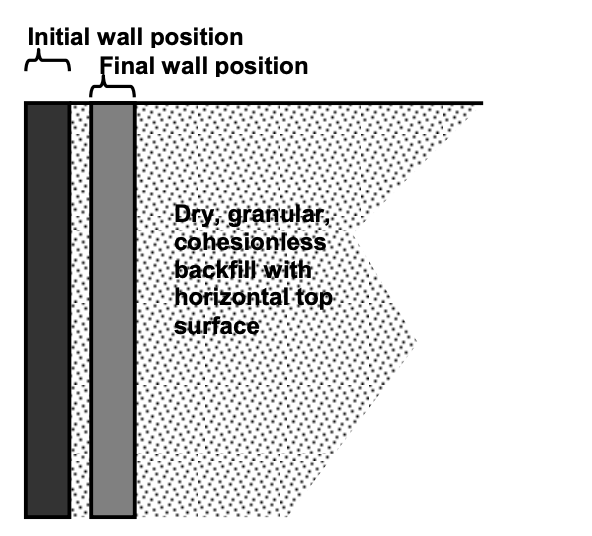
\includegraphics[width=0.3\columnwidth]{figs/Q14.png} 
    \caption{}
    \label{fig:placeholder}
\end{figure}
\begin{enumerate}
\begin{multicols}{2}
\item parallel to the wall face and acting downwards
\item normal to the wall face
\item oblique to the wall face acting downwards
\item oblique to the wall face acting upwards
\end{multicols}
\end{enumerate}

\item An embankment is to be constructed with a granular soil (bulk unit weight $= 20$ kN/m$^3$) on a saturated clayey silt deposit (undrained shear strength $= 25$ kPa). Assuming undrained general shear failure and bearing capacity factor of $5.7$, the maximum height (in m) of the embankment at the point of failure is \hfill \brak{GATE \ CE \ 2012}
\begin{enumerate}
\begin{multicols}{2}
\item $7.1$
\item $5.0$
\item $4.5$
\item $2.5$
\end{multicols}
\end{enumerate}

\item A trapezoidal channel is $10.0$ m wide at the base and has a side slope of $4$ horizontal to $3$ vertical. The bed slope is $0.002$. The channel is lined with smooth concrete \brak{\text{Manning's $n = 0.012$}}. The hydraulic radius \brak{in \ m} for a depth of flow of $3.0$ m is \hfill \brak{GATE \ CE \ 2012}
\begin{enumerate}
\begin{multicols}{2}
\item $20.0$
\item $3.5$
\item $3.0$
\item $2.1$
\end{multicols}
\end{enumerate}

\item A rectangular open channel of width $5.0$ m is carrying a discharge of $100$ m$^3$/s. The Froude number of the flow is $0.8$. The depth of flow (in m) in the channel is \hfill \brak{GATE \ CE \ 2012}
\begin{enumerate}
\begin{multicols}{2}
\item $4$
\item $5$
\item $16$
\item $20$
\end{multicols}
\end{enumerate}

\item The circular water pipes shown are flowing full. The velocity of flow \brak{\text{in m/s}} in the branch pipe "R" is \hfill \brak{GATE \ CE \ 2012}

\begin{figure}[H]
    \centering
    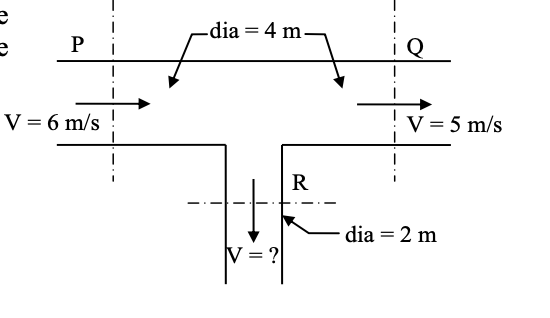
\includegraphics[width=0.3\columnwidth]{figs/Q18.png} 
    \caption{}
    \label{fig:placeholder}
\end{figure}
\begin{enumerate}
\begin{multicols}{2}
\item $3$
\item $4$
\item $5$
\item $6$
\end{multicols}
\end{enumerate}

\item The ratio of actual evapo-transpiration to potential evapo-transpiration is in the range \hfill \brak{GATE \ CE \ 2012}
\begin{enumerate}
\begin{multicols}{2}
\item $0.0$ to $0.4$
\item $0.6$ to $0.9$
\item $0.0$ to $1.0$
\item $1.0$ to $2.0$
\end{multicols}
\end{enumerate}

\item A sample of domestic sewage is digested with silver sulphate, sulphuric acid, potassium dichromate, and mercuric sulphate in chemical oxygen demand \brak{COD} test. The digested sample is titrated with standard ferrous ammonium sulphate \brak{FAS} to determine the un-reacted amount of \hfill \brak{GATE \ CE \ 2012}
\begin{enumerate}
\begin{multicols}{2}
\item mercuric sulphate
\item potassium dichromate
\item silver sulphate
\item sulphuric acid
\end{multicols}
\end{enumerate}

\item Assertion [a]: At a manhole, the crown of the outgoing sewer should not be higher than the crown of the incoming sewer. \\
Reason [r]: Transition from a larger diameter incoming sewer to a smaller diameter outgoing sewer at a manhole should not be made. \hfill \brak{GATE \ CE \ 2012}
\begin{enumerate}
\begin{multicols}{2}
\item Both [a] and [r] are true and [r] is the correct reason for [a]
\item Both [a] and [r] are true but [r] is not the correct reason for [a]
\item Both [a] and [r] are false
\item [a] is true but [r] is false
\end{multicols}
\end{enumerate}

\item Two major roads with two lanes each are crossing in an urban area to form an uncontrolled intersection. The number of conflict points when both roads are one-way is 'X' and when both roads are two-way is 'Y'. The ratio of X to Y is \hfill \brak{GATE \ CE \ 2012}
\begin{enumerate}
\begin{multicols}{2}
\item $0.25$
\item $0.33$
\item $0.50$
\item $0.75$
\end{multicols}
\end{enumerate}

\item Two bitumen samples 'X' and 'Y' have softening points $45^\degree$C and $60^\degree$C, respectively. Consider: \hfill \brak{GATE \ CE \ 2012}
\begin{enumerate}
\item Viscosity of 'X' will be higher than that of 'Y' at the same temperature.
\item Penetration value of 'X' will be less than that of 'Y' under standard conditions.
\end{enumerate}
The CORRECT option evaluating the above statements is
\begin{enumerate}
\begin{multicols}{2}
\item Both I and II are TRUE
\item I is FALSE and II is TRUE
\item Both I and II are FALSE
\item I is TRUE and II is FALSE
\end{multicols}
\end{enumerate}

\item Road roughness is measured using \hfill \brak{GATE \ CE \ 2012}
\begin{enumerate}
\begin{multicols}{2}
\item Benkelman beam
\item Bump integrator
\item Dynamic cone penetrometer
\item Falling weight deflectometer
\end{multicols}
\end{enumerate}



\item Which of the following errors can be eliminated by reciprocal measurements in differential leveling?\\
I Error due to earth's curvature\\
II Error due to atmospheric refraction \hfill \brak{GATE \ CE \ 2012}
\begin{enumerate}
\begin{multicols}{2}
\item Both I and II
\item I only
\item II only
\item Neither I nor II
\end{multicols}
\end{enumerate}


\item The error in 
\begin{align}
    \frac{d}{dx}f(x)\bigg|_{x=x_0}
\end{align} 
for a continuous function estimated with $h=0.03$ using the central difference formula
\begin{align}
\frac{d}{dx}f(x)\bigg|_{x=x_0}\approx\frac{f(x_0+h)-f(x_0-h)}{2h}
\end{align}
is $2\times10^{-3}$. The values of $x_0$ and $f(x_0)$ are $19.78$ and $500.01$, respectively. The corresponding error in the central difference estimate for $h=0.02$ is approximately \hfill \brak{GATE \ CE \ 2012}
\begin{enumerate}
\begin{multicols}{2}
\item $1.3\times10^{-4}$
\item $3.0\times10^{-4}$
\item $4.5\times10^{-4}$
\item $9.0\times10^{-4}$
\end{multicols}
\end{enumerate}

\item In an experiment, positive and negative values are equally likely to occur. The probability of obtaining at most one negative value in five trials is \hfill \brak{GATE \ CE \ 2012}
\begin{enumerate}
\begin{multicols}{2}
\item $\frac{1}{32}$
\item $\frac{2}{32}$
\item $\frac{3}{32}$
\item $\frac{6}{32}$
\end{multicols}
\end{enumerate}

\item The eigenvalues of matrix \myvec{$9$ & $5$ \\ $5$ & $8$} are \hfill \brak{GATE \ CE \ 2012}
\begin{enumerate}
\begin{multicols}{2}
\item $-2.42$ and $6.86$
\item $3.48$ and $13.53$
\item $4.70$ and $6.86$
\item $6.86$ and $9.50$
\end{multicols}
\end{enumerate}

\item For the parallelogram OPQR shown in the sketch, 
\begin{align}
\overrightarrow{OP}=a\hat{i}+b\hat{j} and \overrightarrow{OR}=c\hat{i}+d\hat{j}
\end{align}
.The area of the parallelogram is \hfill \brak{GATE \ CE \ 2012}
\begin{figure}[H]
    \centering
    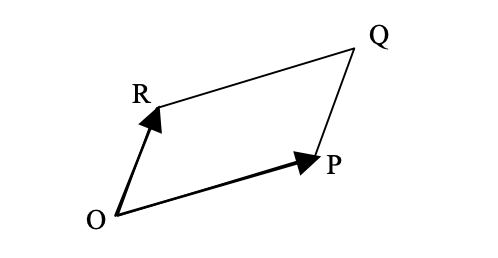
\includegraphics[width=0.3\columnwidth]{figs/Q29.png} 
    \caption{}
    \label{fig:placeholder}
\end{figure}
\begin{enumerate}
\begin{multicols}{2}
\item $a d - b c$
\item $a c + b d$
\item $a d + b c$
\item $a b - c d$
\end{multicols}
\end{enumerate}

\item The solution of the ordinary differential equation $\frac{dy}{dx}+2y=0$ for the boundary condition $y=5$ at $x=1$ is \hfill \brak{GATE \ CE \ 2012}
\begin{enumerate}
\begin{multicols}{2}
\item $y=e^{-2x}$
\item $y=2e^{-2x}$
\item $y=10.95\,e^{-2x}$
\item $y=36.95\,e^{-2x}$
\end{multicols}
\end{enumerate}

\item A simply supported beam is subjected to a uniformly distributed load of intensity $w$ per unit length, on half of the span from one end. The length of the span and the flexural stiffness are denoted as $l$ and $EI$, respectively. The deflection at mid-span of the beam is \hfill \brak{GATE \ CE \ 2012}
\begin{enumerate}
\begin{multicols}{2}
\item $\frac{5\,w\,l^4}{6144\ EI}$
\item $\frac{5\,w\,l^4}{768\ EI}$
\item $\frac{5\,w\,l^4}{384\ EI}$
\item $\frac{5\,w\,l^4}{192\ EI}$
\end{multicols}
\end{enumerate}

\item The sketch shows a column with a pin at the base and rollers at the top. It is subjected to an axial force $P$ and a moment $M$ at mid-height. The reaction at R is/are \hfill \brak{GATE \ CE \ 2012}

\begin{figure}[H]
    \centering
    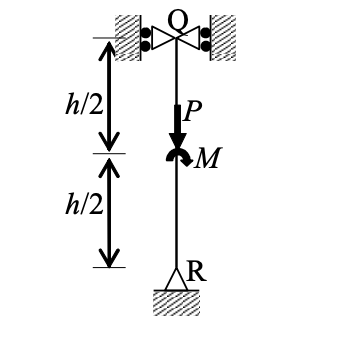
\includegraphics[width=0.3\columnwidth]{figs/Q32.png} 
    \caption{}
    \label{fig:placeholder}
\end{figure}

\begin{enumerate}

\item a vertical force equal to $P$
\item a vertical force equal to $\frac{P}{2}$
\item a vertical force equal to $P$ and a horizontal force equal to $\frac{M}{h}$
\item a vertical force equal to $\frac{P}{2}$ and a horizontal force equal to $\frac{M}{h}$

\end{enumerate}

\item A concrete beam prestressed with a parabolic tendon is shown in the sketch. The eccentricity of the tendon is measured from the centroid of the cross-section. The applied prestressing force at service is $1620$ kN. The uniformly distributed load of $45\ \brak{kN/m}$ includes the self-weight. The stress (in $\text{N/mm}^2$) in the bottom fibre at mid-span is \hfill \brak{GATE \ CE \ 2012}
\begin{figure}[H]
    \centering
    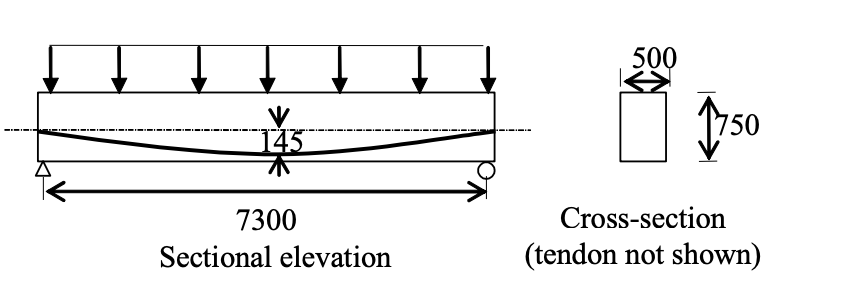
\includegraphics[width=0.3\columnwidth]{figs/Q33.png} 
    \caption{}
    \label{fig:placeholder}
\end{figure}

\begin{enumerate}
\begin{multicols}{2}
\item tensile $2.90$
\item compressive $2.90$
\item tensile $4.32$
\item compressive $4.32$
\end{multicols}
\end{enumerate}

\item A symmetric frame PQR consists of two inclined members PQ and QR, connected at 'Q' with a rigid joint, and hinged at 'P' and 'R'. The horizontal length PR is $l$. If a weight $W$ is suspended at 'Q', the bending moment at 'Q' is \hfill \brak{GATE \ CE \ 2012}
\begin{enumerate}
\begin{multicols}{4}
\item $\frac{Wl}{2}$
\item $\frac{Wl}{4}$
\item $\frac{Wl}{8}$
\item zero
\end{multicols}
\end{enumerate}

\item Two plates are connected by fillet welds of size $10$ mm and subjected to tension, as shown in the sketch. The thickness of each plate is $12\ \text{mm}$. The yield stress and the ultimate tensile stress of steel are $250\ \text{MPa}$ and $410\ \text{MPa}$, respectively. The welding is done in the workshop ($\gamma_{mw}=1.25$). As per IS 800:2007 (Limit State Method), the minimum length \brak{\text{rounded up to nearest higher multiple of $5\ \text{mm}$}} of each weld to transmit $P=270\ \text{kN}$ is \hfill \brak{GATE \ CE \ 2012}

\begin{figure}[H]
    \centering
    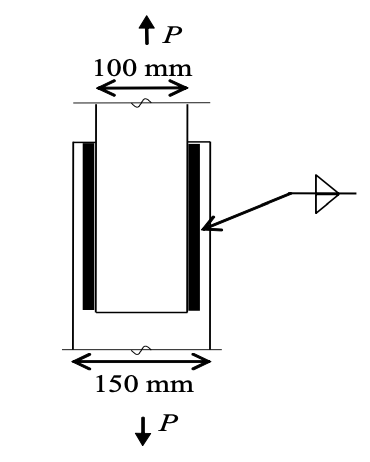
\includegraphics[width=0.3\columnwidth]{figs/Q35.png} 
    \caption{}
    \label{fig:placeholder}
\end{figure}
\begin{enumerate}
\begin{multicols}{2}
\item $100\ \text{mm}$
\item $105\ \text{mm}$
\item $110\ \text{mm}$
\item $115\ \text{mm}$
\end{multicols}
\end{enumerate}

\item Two soil specimens with identical geometric dimensions were subjected to falling head permeability tests under identical conditions. The ratio of initial to final water heads for the test involving the first specimen was $1.25$. If the coefficient of permeability of the second specimen is five times that of the first, the ratio of initial to final water heads in the test involving the second specimen is \hfill \brak{GATE \ CE \ 2012}
\begin{enumerate}
\begin{multicols}{2}
\item $3.05$
\item $3.80$
\item $4.00$
\item $6.25$
\end{multicols}
\end{enumerate}

\item A layer of normally consolidated, saturated silty clay of $1\ \text{m}$ thickness is subjected to one-dimensional consolidation under a pressure increment of $20\ \text{kPa}$. Properties: specific gravity $=2.7$, natural moisture content $=45\%$, compression index $=0.45$, recompression index $=0.05$. Initial average effective stress within layer $=100\ \text{kPa}$. Assuming Terzaghi's theory, the primary consolidation settlement \brak{nearest \ mm} is \hfill \brak{GATE \ CE \ 2012}
\begin{enumerate}
\begin{multicols}{2}
\item $2$ mm
\item $9$ mm
\item $14$ mm
\item $16$ mm
\end{multicols}
\end{enumerate}

\item Steady state seepage is taking place through a soil element at $Q$, $2\ \text{m}$ below ground surface immediately downstream of the toe of an earthen dam \brak{see \ sketch}. The water level in a piezometer at $P$ \brak{500 \ mm \ above \ Q} is at ground surface. The water level in a piezometer at $R$ \brak{500 \ mm \ below \ Q} is $100\ \text{mm}$ above ground surface. Bulk saturated unit weight $=18\ \text{kN/m}^3$, unit weight of water $=9.81\ \text{kN/m}^3$. The vertical effective stress \brak{in \ kPa} at $Q$ is \hfill \brak{GATE \ CE \ 2012}

\begin{figure}[H]
    \centering
    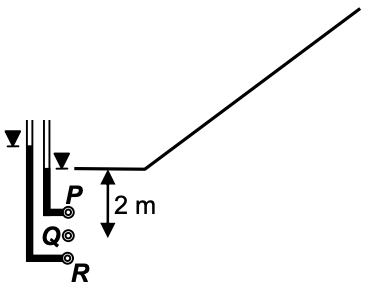
\includegraphics[width=0.3\columnwidth]{figs/Q38.png} 
    \caption{}
    \label{fig:placeholder}
\end{figure}

\begin{enumerate}
\begin{multicols}{2}
\item $14.42$
\item $15.89$
\item $16.38$
\item $18.34$
\end{multicols}
\end{enumerate}

\item The top width and the depth of flow in a triangular channel were measured as $4\ \text{m}$ and $1\ \text{m}$, respectively. The measured velocities on the centre line at the water surface, $0.2\ \text{m}$ and $0.8\ \text{m}$ below the surface are $0.7\ \text{m/s}$, $0.6\ \text{m/s}$ and $0.4\ \text{m/s}$ respectively. Using two-point method of velocity measurement, the discharge (in $\text{m}^3/\text{s}$) in the channel is \hfill \brak{GATE \ CE \ 2012}
\begin{enumerate}
\begin{multicols}{2}
\item $1.4$
\item $1.2$
\item $1.0$
\item $0.8$
\end{multicols}
\end{enumerate}

\item Group I contains parameters and Group II lists methods/instruments.\\
Group I: P. Streamflow velocity \quad Q. Evapo-transpiration rate \quad R. Infiltration rate \quad S. Wind velocity\\
Group II: 1. Anemometer \quad 2. Penman's method \quad 3. Horton's method \quad 4. Current meter\\
The CORRECT match of Group I with Group II is \hfill \brak{GATE \ CE \ 2012}
\begin{enumerate}
\begin{multicols}{2}
\item P-1, Q-2, R-3, S-4
\item P-4, Q-3, R-2, S-1
\item P-4, Q-2, R-3, S-1
\item P-1, Q-3, R-2, S-4
\end{multicols}
\end{enumerate}

\item Wheat crop requires $55$ cm of water during $120$ days of base period. Total rainfall during this period is $100$ mm. Assume irrigation efficiency $=60\%$. The area (in ha) of land that can be irrigated with canal flow $0.01$ m$^{3}$/s is \hfill \brak{GATE \ CE \ 2012}
\begin{enumerate}
\begin{multicols}{2}
\item $13.82$
\item $18.85$
\item $23.04$
\item $230.40$
\end{multicols}
\end{enumerate}

\item A water sample has a pH of $9.25$. The concentration of hydroxyl ions in the water sample is \hfill \brak{GATE \ CE \ 2012}
\begin{enumerate}
\begin{multicols}{2}
\item $10^{-9.25}\ \text{moles/L}$
\item $10^{-4.75}\ \text{mmoles/L}$
\item $0.302\ \text{mg/L}$
\item $3.020\ \text{mg/L}$
\end{multicols}
\end{enumerate}


\item A town is required to treat $4.2$ m$^{3}$/min of raw water for daily domestic supply. Flocculating particles are to be produced by chemical coagulation. A column analysis indicated that an overflow rate of $0.2$ mm/s will produce satisfactory particle removal in a settling basin at a depth of $3.5$ m. The required surface area \brak{\text{in  m$^{2}$}} for settling is \hfill \brak{GATE \ CE \ 2012}
\begin{enumerate}
\begin{multicols}{2}
\item $210$
\item $350$
\item $1728$
\item $21000$
\end{multicols}
\end{enumerate}

\item A pavement designer has arrived at a design traffic of $100$ million standard axles for a newly developing national highway as per IRC:37 guidelines using the following data: design life $=15$ years, commercial vehicle count before pavement construction $=4500$ vehicles/day, annual traffic growth rate $=8\%$. The vehicle damage factor used in the calculation was \hfill \brak{GATE \ CE \ 2012}
\begin{enumerate}
\begin{multicols}{2}
\item $1.53$
\item $2.24$
\item $3.66$
\item $4.14$
\end{multicols}
\end{enumerate}

\item The following data are related to a horizontal curved portion of a two-lane highway: length of curve $=200$ m, radius of curve $=300$ m and width of pavement $=7.5$ m. In order to provide a stopping sight distance \brak{SSD} of $80$ m, the set back distance (in m) required from the centre line of the inner lane of the pavement is \hfill \brak{GATE \ CE \ 2012}
\begin{enumerate}
\begin{multicols}{2}
\item $2.54$
\item $4.55$
\item $7.10$
\item $7.96$
\end{multicols}
\end{enumerate}

\item A two-lane urban road with one-way traffic has a maximum capacity of $1800$ vehicles/hour. Under the jam condition, the average length occupied by the vehicles is $5.0$ m. The speed versus density relationship is linear. For a traffic volume of $1000$ vehicles/hour, the density \brak{in vehicles/km} is \hfill \brak{GATE \ CE \ 2012}
\begin{enumerate}
\begin{multicols}{2}
\item $52$
\item $58$
\item $67$
\item $75$
\end{multicols}
\end{enumerate}

\item The horizontal distance between two stations P and Q is $100$ m. The vertical angles from P and Q to the top of a vertical tower at T are $3^\degree$ and $5^\degree$ above horizontal, respectively. The vertical angles from P and Q to the base of the tower are $0.1^\degree$ and $0.5^\degree$ below horizontal, respectively. Stations P, Q and the tower are in the same vertical plane with P and Q being on the same side of T. Neglecting earth's curvature and atmospheric refraction, the height \brak{in \ m} of the tower is \hfill \brak{GATE \ CE \ 2012}
\begin{enumerate}
\begin{multicols}{2}
\item $6.972$
\item $12.387$
\item $12.540$
\item $128.745$
\end{multicols}
\end{enumerate}


\textbf{Common Data for Questions 48 and 49}

The flow net around a sheet pile wall is shown in the
sketch. The properties of the soil are: permeability
coefficient = $0.09$ m/day \brak{isotropic}, specific gravity
= $2.70$ and void ratio = $0.85$. The sheet pile wall and
the bottom of the soil are impermeable.
\begin{figure}[H]
    \centering
    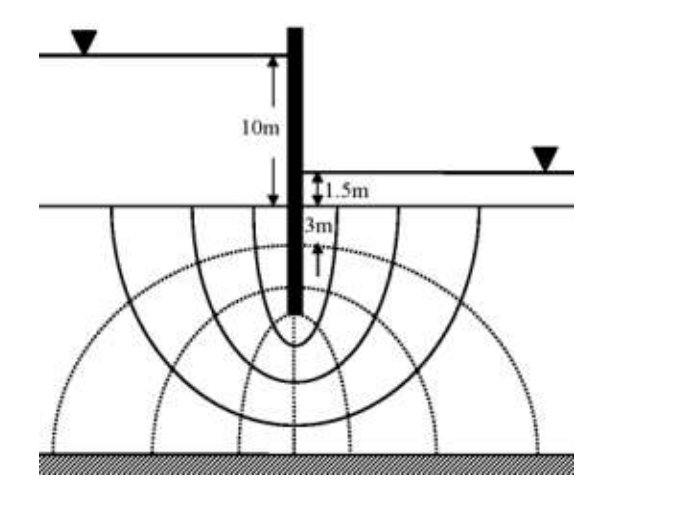
\includegraphics[width=0.3\columnwidth]{figs/Q48.png} 
    \caption{}
    \label{fig:placeholder}
\end{figure}
\item The seepage loss \brak{\text{in m$^{3}$ per day per unit length of the wall}} of water is \hfill \brak{GATE \ CE \ 2012}
\begin{enumerate}
\begin{multicols}{2}
\item $0.33$
\item $0.38$
\item $0.43$
\item $0.54$
\end{multicols}
\end{enumerate}

\item The factor of safety against the occurrence of piping failure is \hfill \brak{GATE \ CE \ 2012}
\begin{enumerate}
\begin{multicols}{2}
\item $3.55$
\item $2.93$
\item $2.60$
\item $0.39$
\end{multicols}
\end{enumerate}


\textbf{Common Data for Questions 50 and 51}

\begin{figure}[H]
    \centering
    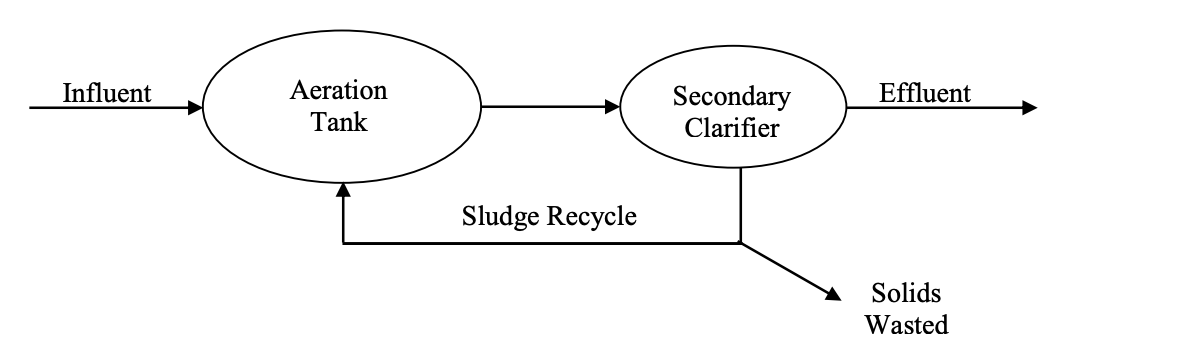
\includegraphics[width=0.3\columnwidth]{figs/Q50.png} 
    \caption{}
    \label{fig:placeholder}
\end{figure}

An activated sludge system \brak{sketched \ below} is operating at equilibrium with the following information. Wastewater related data: flow rate = 500 m$^{3}$ /hour, influent BOD = $150$ mg/L, effluent BOD = $10$ mg/L. Aeration tank related data: hydraulic retention time = $8$ hours, mean cell-residence time = $240$ hours, volume = $4000$ m$^{3}$ , mixed liquor suspended solids = $2000$ mg/L. 

\item The food-to-biomass \brak{F/M} ratio \brak{in \ kg \ BOD \ per \ kg \ biomass \ per \ day} for the aeration tank is \hfill \brak{GATE \ CE \ 2012}
\begin{enumerate}
\begin{multicols}{2}
\item $0.015$
\item $0.210$
\item $0.225$
\item $0.240$
\end{multicols}
\end{enumerate}

\item The mass \brak{in \ kg/day} of solids wasted from the system is \hfill \brak{GATE \ CE \ 2012}
\begin{enumerate}
\begin{multicols}{2}
\item $24000$
\item $1000$
\item $800$
\item $33$
\end{multicols}
\end{enumerate}

\textbf{Linked Answer Questions}

\textbf{Statement for Linked Answer Questions 52 and 53}

\begin{figure}[H]
    \centering
    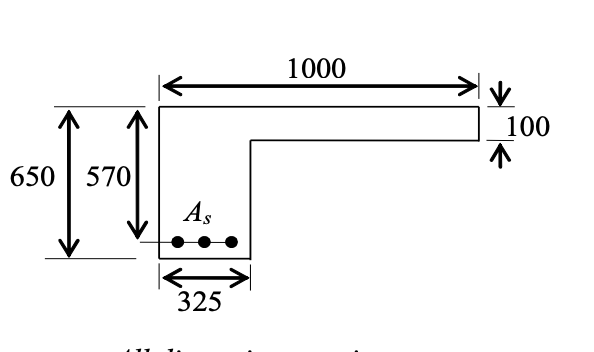
\includegraphics[width=0.3\columnwidth]{figs/Q52.png} 
    \caption{}
    \label{fig:placeholder}
\end{figure}

The cross-section at mid-span of a beam at the edge of
a slab is shown in the sketch. A portion of the slab is
considered as the effective flange width for the beam.
The grades of concrete and reinforcing steel are $M25$
and $Fe415$, respectively. The total area of reinforcing
bars \brak{As} is $4000$ mm$^{2}$
. At the ultimate limit state, xu
denotes the depth of the neutral axis from the top
fibre. Treat the section as under-reinforced and
flanged (xu $>$ $100$ mm).

\item The value of $x_u$ (in mm) computed as per the Limit State Method of IS $456$:$2000$ is \hfill \brak{GATE \ CE \ 2012}
\begin{enumerate}
\begin{multicols}{2}
\item $200.0$
\item $223.3$
\item $236.3$
\item $273.6$
\end{multicols}
\end{enumerate}

\item The ultimate moment capacity \brak{in \ kNm} of the section, as per the Limit State Method of IS $456$ : $2000$ is \hfill \brak{GATE \ CE \ 2012}
\begin{enumerate}
\begin{multicols}{2}
\item $475.2$
\item $717.0$
\item $756.4$
\item $762.5$
\end{multicols}
\end{enumerate}


\textbf{Statement for Linked Answer Questions 54 and 55}

The drainage area of a watershed is 50 km$^{2}$. The $\phi$ index is $0.5$ cm/hour and the base flow at the outlet is
$10$ m$^3$/s. One hour unit hydrograph (unit depth = $1$ cm) of the watershed is triangular in shape with a time base of $15$ hours. The peak ordinate occurs at $5$ hours.

\item The peak ordinate (in m$^{3}$/s/cm) of the unit hydrograph is \hfill \brak{GATE \ CE \ 2012}
\begin{enumerate}
\begin{multicols}{2}
\item $10.00$
\item $18.52$
\item $37.03$
\item $185.20$
\end{multicols}
\end{enumerate}

\item For a storm of depth of $5.5$ cm and duration of $1$ hour, the peak ordinate (in m$^{3}$/s) of the hydrograph is \hfill \brak{GATE \ CE \ 2012}
\begin{enumerate}
\begin{multicols}{2}
\item $55.00$
\item $82.60$
\item $92.60$
\item $102.60$
\end{multicols}
\end{enumerate}

\textbf{General Aptitude (GA) Questions}
\section*{Q. $56$ - Q. $60$ carry one mark each}

\item Despite several \underline{\hspace{1.7cm}} the mission succeeded in its attempt to resolve the conflict. \hfill \brak{GATE \ CE \ 2012}
\begin{enumerate}
\begin{multicols}{2}
\item attempts
\item setbacks
\item meetings
\item delegations
\end{multicols}
\end{enumerate}

\item The cost function for a product in a firm is given by $5q^2$, where $q$ is the amount of production. The firm can sell the product at a market price of $50$ per unit. The number of units to be produced by the firm such that the profit is maximized is \hfill \brak{GATE \ CE \ 2012}
\begin{enumerate}
\begin{multicols}{2}
\item $5$
\item $10$
\item $15$
\item $25$
\end{multicols}
\end{enumerate}

\item Suresh's dog is the one \underline{\hspace{1.7cm}} was hurt in the stampede. \hfill \brak{GATE \ CE \ 2012}
\begin{enumerate}
\begin{multicols}{2}
\item that
\item which
\item who
\item whom
\end{multicols}
\end{enumerate}

\item Choose the grammatically INCORRECT sentence: \hfill \brak{GATE \ CE \ 2012}
\begin{enumerate}
\item They gave us the money back less the service charges of Three Hundred rupees.
\item This country's expenditure is not less than that of Bangladesh.
\item The committee initially asked for a funding of Fifty Lakh rupees, but later settled for a lesser sum.
\item This country's expenditure on educational reforms is very less.
\end{enumerate}

\item Which one of the following options is the closest in meaning to the word given below? \\
Mitigate \hfill \brak{GATE \ CE \ 2012}
\begin{enumerate}
\begin{multicols}{2}
\item Diminish
\item Divulge
\item Dedicate
\item Denote
\end{multicols}
\end{enumerate}

\section*{Q. $61$ - Q. $65$ carry two marks each}

\item A political party orders an arch for the entrance to the ground in which the annual convention is being held. The profile of the arch follows the equation y = 2x - 0.1x$^{2}$ where $y$ is the height of the arch in meters. The maximum possible height of the arch is \hfill \brak{GATE \ CE \ 2012}
\begin{enumerate}
\begin{multicols}{2}
\item $8$
\item $10$
\item $12$
\item $14$
\end{multicols}
\end{enumerate}

\item Wanted Temporary, Part-time persons for the post of Field Interviewer to conduct personal interviews to collect and collate economic data. Requirements: High School-pass, must be available for Day, Evening and Saturday work. Transportation paid, expenses reimbursed. The best inference from the above advertisement is \hfill \brak{GATE \ CE \ 2012}
\begin{enumerate}
\begin{multicols}{2}
\item Gender-discriminatory
\item Xenophobic
\item Not designed to make the post attractive
\item Not gender-discriminatory
\end{multicols}
\end{enumerate}

\item Given the sequence of terms, AD  CG  FK  JP, the next term is \hfill \brak{GATE \ CE \ 2012}
\begin{enumerate}
\begin{multicols}{2}
\item OV
\item OW
\item PV
\item PW
\end{multicols}
\end{enumerate}

\item Which of the following assertions are CORRECT? \\
P: Adding $7$ to each entry in a list adds $7$ to the mean of the list \\
Q: Adding $7$ to each entry in a list adds $7$ to the standard deviation of the list \\
R: Doubling each entry in a list doubles the mean of the list \\
S: Doubling each entry in a list leaves the standard deviation of the list unchanged \hfill \brak{GATE \ CE \ 2012}
\begin{enumerate}
\begin{multicols}{2}
\item P, Q
\item Q, R
\item P, R
\item R, S
\end{multicols}
\end{enumerate}

\item An automobile plant contracted to buy shock absorbers from two suppliers X and Y. X supplies $60\%$ and Y supplies $40\%$ of the shock absorbers. All shock absorbers are subjected to a quality test. The ones that pass are considered reliable. Of X's shock absorbers, $96\%$ are reliable. Of Y's shock absorbers, $72\%$ are reliable. The probability that a randomly chosen shock absorber, which is found to be reliable, is made by Y is \hfill \brak{GATE \ CE \ 2012}
\begin{enumerate}
\begin{multicols}{2}
\item $0.288$
\item $0.334$
\item $0.667$
\item $0.720$
\end{multicols}
\end{enumerate}


\end{enumerate}
\end{document}